\pdfbookmark{Общая характеристика работы}{characteristic}             % Закладка pdf
\section*{Общая характеристика работы}

\newcommand{\actuality}{\pdfbookmark[1]{Актуальность}{actuality}\underline{\textbf{\actualityTXT}}}
\newcommand{\progress}{\pdfbookmark[1]{Разработанность темы}{progress}\underline{\textbf{\progressTXT}}}
\newcommand{\aim}{\pdfbookmark[1]{Цели}{aim}\underline{{\textbf\aimTXT}}}
\newcommand{\tasks}{\pdfbookmark[1]{Задачи}{tasks}\underline{\textbf{\tasksTXT}}}
\newcommand{\aimtasks}{\pdfbookmark[1]{Цели и задачи}{aimtasks}\aimtasksTXT}
\newcommand{\novelty}{\pdfbookmark[1]{Научная новизна}{novelty}\underline{\textbf{\noveltyTXT}}}
\newcommand{\thInfluence}{\pdfbookmark[1]{Теоретическая значимость}{thInfluence}\underline{\textbf{\thInfluenceTXT}}}
\newcommand{\prInfluence}{\pdfbookmark[1]{Практическая значимость}{prInfluence}\underline{\textbf{\prInfluenceTXT}}}
\newcommand{\methods}{\pdfbookmark[1]{Методология и методы исследования}{methods}\underline{\textbf{\methodsTXT}}}
\newcommand{\defpositions}{\pdfbookmark[1]{Положения, выносимые на защиту}{defpositions}\underline{\textbf{\defpositionsTXT}}}
\newcommand{\reliability}{\pdfbookmark[1]{Достоверность}{reliability}\underline{\textbf{\reliabilityTXT}}}
\newcommand{\probation}{\pdfbookmark[1]{Апробация}{probation}\underline{\textbf{\probationTXT}}}
\newcommand{\contribution}{\pdfbookmark[1]{Личный вклад}{contribution}\underline{\textbf{\contributionTXT}}}
\newcommand{\publications}{\pdfbookmark[1]{Публикации}{publications}\underline{\textbf{\publicationsTXT}}}


{\actuality} Тематическое моделирование --- метод анализа текстов, производящий мягкую кластеризацию как слов, так и документов. У тематического моделирования есть два важных свойства, отличающих его от других методов работы с текстами. 

Во-первых, тренировка модели происходит ``без учителя'': для того, чтобы обработать корпус текстов посредством тематического моделирования не требуется размеченных данных или предобученных моделей. Это позволяет использовать тематическое моделирование в задачах, использование в которых предобученных моделей затрудненно: для анализа узкоспецифических текстов или текстов на редких языках, для анализа тексто-подобных данных (программный код, тексты песен, банковские транзакции, географические данные, музыкальные произведения).

Во-вторых, результатом работы тематической модели являются \textit{темы}, описываемые вероятностными распределениями. Компоненты этих распределений --- вероятность слова с учётом темы и вероятность темы в документе --- прозрачны и играют понятную роль в модели. 
Зачастую эксперт может связать тему (как множество слов и множество документов) с каким-либо понятием из предметной области (т.е. проинтерпретировать её); такое осознание помогает пониманию структуры коллекции. Поэтому важное применение тематического моделирования --- помощь в понимании больших массивов неструктурированных данных.

Аддитивная Регуляризация Тематических это такой подход который даёт много гибкости.

\textbf{Степень разработанности темы исследования}. 

Подбор гиперпараметров. Доступность. Подстраховка от заблуждений.

Всё это является нерешёнными проблемами.

% {\progress}
% Этот раздел должен быть отдельным структурным элементом по
% ГОСТ, но он, как правило, включается в описание актуальности
% темы. Нужен он отдельным структурынм элемементом или нет ---
% смотрите другие диссертации вашего совета, скорее всего не нужен.

{\aim} данного диссертационного исследования является разработка методов построения интерпретируемых тематических моделей, применимых для широкого ряда задач. Проделанная работа опубликована на GitHub как открытая библиотека TopicNet.

Для~достижения поставленной цели решаются следующие {\tasks}:
\begin{enumerate}[beginpenalty=10000] % https://tex.stackexchange.com/a/476052/104425
  \item кластеризация интентов при помощи специального куба
  \item изучение принятых метрик интерпретируемости
  \item введение кастомных метрик качества
  \item введение кастомных регуляризаторов
  \item перформанс бэзлайна сравнивается с генсимом и рецептом Мурата
\end{enumerate}

{\novelty}
\begin{enumerate}[beginpenalty=10000] % https://tex.stackexchange.com/a/476052/104425
  \item Впервые \ldots
  \item Впервые \ldots
  \item Было выполнено оригинальное исследование \ldots
\end{enumerate}

{\influence} 
Абзац про нужность библиотеки ТопикНет

Абзац про пользу относительных коэффициентов

Абзац про применимость всего этого в таких-то задачах.


{\methods} В работе использованы методы теории вероятностей, оптимизации, NLP. Экспериментальное исследование проводится на языке Python; опубликованная на GitHub библиотека TopicNet, подытоживающая результаты исследования открыта для широкой публики и удовлетворяет принципам воспроизводимости результатов.

{\defpositions}
\begin{enumerate}[beginpenalty=10000] % https://tex.stackexchange.com/a/476052/104425
  \item Изучение репрезентативности имеющихся мер интерпретируемости
  \item Предложены относительные веса модальностей, и относительные коэффициенты сглаживания/разреживания. Обеспечивают переносимость тематических моделей. Отличаются от аналогов...
  \item Псевдорегуляризатор, обеспечивающий быстрое однопроходное вычисление векторизации документов. Отличается от аналогов тем, что улучшает многие меры качества.
  \item Концепция дерева эксперимента и кубов в библиотеке TopicNet
  \item Новая адаптивная стратегия регуляризации, реализованная как отдельный куб в TopicNet
\end{enumerate}


{\reliability} полученных результатов обеспечивается \ldots 

{\probation}
Основные результаты диссертации докладывались на следующих конференциях и семинарах:
\begin{itemize}
    \item Международная конференция по компьютерной лингвистике “Диалог”, Москва, 1 июня 2018.
    \item International Conference Recent Advances in Natural Language Processing (RANLP), Варна, 3 сентября 2019.
    \item Открытая лекция в рамках образовательного проекта Физтех.Рост, Долгопрудный, 18 октября 2019.
    \item Научный семинар про коэффициентов
    \item Научный семинар про ТопикНет
    \item OpenTalks.AI – ведущая независимая открытая конференция по искусственному интеллекту, Москва, 20 февраля 2020 года.
    \item International Conference on Language Resources and Evaluation (LREC), Марсель (должна была состоятся в мае 2020).
\end{itemize}

{\contribution} Автор принимал активное участие \ldots

\ifnumequal{\value{bibliosel}}{0}
{%%% Встроенная реализация с загрузкой файла через движок bibtex8. (При желании, внутри можно использовать обычные ссылки, наподобие `\cite{vakbib1,vakbib2}`).
    {\publications} Основные результаты по теме диссертации изложены
    в~XX~печатных изданиях,
    X из которых изданы в журналах, рекомендованных ВАК,
    X "--- в тезисах докладов.
}%
{%%% Реализация пакетом biblatex через движок biber
    \begin{refsection}[bl-author, bl-registered]
        % Это refsection=1.
        % Процитированные здесь работы:
        %  * подсчитываются, для автоматического составления фразы "Основные результаты ..."
        %  * попадают в авторскую библиографию, при usefootcite==0 и стиле `\insertbiblioauthor` или `\insertbiblioauthorgrouped`
        %  * нумеруются там в зависимости от порядка команд `\printbibliography` в этом разделе.
        %  * при использовании `\insertbiblioauthorgrouped`, порядок команд `\printbibliography` в нём должен быть тем же (см. biblio/biblatex.tex)
        %
        % Невидимый библиографический список для подсчёта количества публикаций:
        \ifxetexorluatex\selectlanguage{english}\fi
        \printbibliography[heading=nobibheading, section=1, env=countauthorvak,          keyword=biblioauthorvak]%
        \printbibliography[heading=nobibheading, section=1, env=countauthorwos,          keyword=biblioauthorwos]%
        \printbibliography[heading=nobibheading, section=1, env=countauthorscopus,       keyword=biblioauthorscopus]%
        \printbibliography[heading=nobibheading, section=1, env=countauthorconf,         keyword=biblioauthorconf]%
        \printbibliography[heading=nobibheading, section=1, env=countauthorother,        keyword=biblioauthorother]%
        \printbibliography[heading=nobibheading, section=1, env=countregistered,         keyword=biblioregistered]%
        \printbibliography[heading=nobibheading, section=1, env=countauthorpatent,       keyword=biblioauthorpatent]%
        \printbibliography[heading=nobibheading, section=1, env=countauthorprogram,      keyword=biblioauthorprogram]%
        \printbibliography[heading=nobibheading, section=1, env=countauthor,             keyword=biblioauthor]%
        \printbibliography[heading=nobibheading, section=1, env=countauthorvakscopuswos, filter=vakscopuswos]%
        \printbibliography[heading=nobibheading, section=1, env=countauthorscopuswos,    filter=scopuswos]%
        %
        \nocite{*}\ifxetexorluatex\selectlanguage{russian}\fi%
        %
        \nocite{intracoh, popov_hier, bulatov2020topicnet, thetaless, prog_cook, prog_view}
        
        {\publications} Основные результаты по теме диссертации изложены в~\arabic{citeauthor}~печатных изданиях,
        \arabic{citeauthorvak} из которых изданы в журналах, рекомендованных ВАК\sloppy%
        \ifnum \value{citeauthorscopuswos}>0%
            , \arabic{citeauthorscopuswos} "--- в~периодических научных журналах, индексируемых Web of~Science и Scopus\sloppy%
        \fi%
        \ifnum \value{citeauthorconf}>0%
            , \arabic{citeauthorconf} "--- в~тезисах докладов.
        \else%
            .
        \fi%
        \ifnum \value{citeregistered}=1%
            \ifnum \value{citeauthorpatent}=1%
                Зарегистрирован \arabic{citeauthorpatent} патент.
            \fi%
            \ifnum \value{citeauthorprogram}=1%
                Зарегистрирована \arabic{citeauthorprogram} программа для ЭВМ.
            \fi%
        \fi%
        \ifnum \value{citeregistered}>1%
            Зарегистрированы\ %
            \ifnum \value{citeauthorpatent}>0%
            \formbytotal{citeauthorpatent}{патент}{}{а}{}\sloppy%
            \ifnum \value{citeauthorprogram}=0 . \else \ и~\fi%
            \fi%
            \ifnum \value{citeauthorprogram}>0%
            \formbytotal{citeauthorprogram}{программ}{а}{ы}{} для ЭВМ.
            \fi%
        \fi%
        % К публикациям, в которых излагаются основные научные результаты диссертации на соискание учёной
        % степени, в рецензируемых изданиях приравниваются патенты на изобретения, патенты (свидетельства) на
        % полезную модель, патенты на промышленный образец, патенты на селекционные достижения, свидетельства
        % на программу для электронных вычислительных машин, базу данных, топологию интегральных микросхем,
        % зарегистрированные в установленном порядке.(в ред. Постановления Правительства РФ от 21.04.2016 N 335)
    \end{refsection}%
    \begin{refsection}[bl-author, bl-registered]
        % Это refsection=2.
        % Процитированные здесь работы:
        %  * попадают в авторскую библиографию, при usefootcite==0 и стиле `\insertbiblioauthorimportant`.
        %  * ни на что не влияют в противном случае
        \nocite{intracoh}
        \nocite{popov_hier}
        \nocite{bulatov2020topicnet}
        \nocite{thetaless}
        \nocite{prog_cook}
        \nocite{prog_view}
        
    \end{refsection}%
        %
        % Всё, что вне этих двух refsection, это refsection=0,
        %  * для диссертации - это нормальные ссылки, попадающие в обычную библиографию
        %  * для автореферата:
        %     * при usefootcite==0, ссылка корректно сработает только для источника из `external.bib`. Для своих работ --- напечатает "[0]" (и даже Warning не вылезет).
        %     * при usefootcite==1, ссылка сработает нормально. В авторской библиографии будут только процитированные в refsection=0 работы.
}


% Для добавления в список публикаций автора работ, которые не были процитированы в
% автореферате, требуется их~перечислить с использованием команды \verb!\nocite! в
% \verb!Synopsis/content.tex!.
 % Характеристика работы по структуре во введении и в автореферате не отличается (ГОСТ Р 7.0.11, пункты 5.3.1 и 9.2.1), потому её загружаем из одного и того же внешнего файла, предварительно задав форму выделения некоторым параметрам

%Диссертационная работа была выполнена при поддержке грантов \dots

\underline{\textbf{Объем и структура работы.}} Диссертация состоит из введения, двух обзорных глав, четырёх глав с результатами проведенного исследования, заключения и библиографии. Полный объём диссертации составляет 143 страницы, включая 17 рисунков и 12 таблиц. Список литературы содержит 154 наименования.

\pdfbookmark{Содержание работы}{description}                          % Закладка pdf
\section*{Содержание работы}
Во \underline{\textbf{введении}} отражается актуальность
исследований, проводимых в~рамках данной диссертационной работы,
приводится обзор научной литературы по~изучаемой проблеме,
формулируется цель, ставятся задачи работы, определяется научная новизна, практическая и теоретическая значимости представляемой работы. Приводится список публикаций автора по теме диссертации и формулируются положения, вносимые на защиту.

\underline{\textbf{Первая глава}} посвящена постановке задачи тематического моделирования. Рассмотрены основные подходы к тематическому моделированию и подробно описан математический аппарат подхода ARTM.

Задача тематического моделирования заключается в нахождении матрицы $\Phi$, содержащей дискретные распределения вероятности слов для каждой темы, и матрицы $\Theta$, содержащей дискретные распределения вероятности тем для каждого документа. Основное требование к модели заключается в том, что произведение этих двух матриц должно приближать распределения вероятности слов для каждого документа. Подход ARTM позволяет вводить различные дополнительные требования к матрицам $\Phi$ и $\Theta$.

В рамках ARTM тематические модели строятся при помощи \textit{EM-алгоритма}, в котором текущие значения матриц $\Phi$ и $\Theta$ итеративно обновляются по определённым формулам. Введение каждого дополнительного регуляризатора приводит к появлению в этих формулах новых слагаемых, не меняющих общую структуру EM-алгоритма. Его программная реализация может быть выполнена один раз в самом общем виде, при этом каждый регуляризатор реализуется независимо от остальных в виде отдельного модуля.

Область применения, уникальная для тематических моделей --- описание коллекции, дающее общее представление о тематической кластерной структуре больших объёмов данных. Зачастую исследователь ищет ответы на вопросы о структуре и природе коллекции, а функция тематической модели как модели языка, способной предсказывать слова в тексте, интересует его меньше.

Приложения тематического моделирования в различных областях наталкиваются на проблемы плохой интерпретируемости тем, дублирующих, мусорных и вводящих в заблуждение тем, неустойчивости результатов моделирования. 

Большую часть этих проблем можно разрешить при помощи настройки гиперпараметров, однако в практико-ориентированной литературе не хватает хорошо проработанной систематической методологии настройки гиперпараметров. В~большинстве работ ограничиваются подбором числа тем и ещё одного-двух гиперпараметров по грубым сеткам значений.  

Сложность подбора гиперпараметров у многокритериальных моделей вызывает необходимость как измерения, так и оптимизации качества тематических моделей одновременно по множеству критериев.

\underline{\textbf{Во второй главе}} рассматриваются критерии качества тематических моделей, используемые в литературе. Проведена категоризация распространённых подходов к измерению качества. Особое внимание уделяется мерам качества, связанными с анализом верхних (наиболее частотных, вероятных, <<топовых>>, top-10) токенов в темах.

\underline{\textbf{Третья глава}} посвящена анализу общих недостатков этих мер качества. Большинство используемых в литературе подходов к оценке интерпретируемости тем укладываются в следующую схему:

\begin{enumerate}
    \item Для каждой темы выбирается какой-то небольшой набор характеризующих её токенов (как правило, это 10 верхних токенов).
    \item{Этот набор анализируется одним из двух способов:
    \begin{itemize}
        \item качество тем оценивается экспертом визуально по этим токенам;
        \item качество тем оценивается путём автоматического вычисления определённых статистик, в частности, парной сочетаемости верхних токенов в текстовой коллекции.
    \end{itemize}
    }
\end{enumerate}

В пункте (1) вышеописанной схемы тема фактически подменяется небольшим списком её верхних токенов. Каким бы образом ни проводился дальнейший анализ, обоснование качества тематической модели после такой подмены представляется проблематичным.

Рисунок \ref{fig:ch3_doc_compound_auto} демонстрирует то, что верхние токены покрывают исчезающе малую часть коллекции, и ситуация ещё более усложняется наличием дополнительного требования парной сочетаемости токенов в окне. Численные расчёты подтверждают, что когерентность отдельно взятой темы, в большинстве случаев, учитывает менее тысячной доли всего корпуса текста.

\begin{figure}
    %\begin{tabular}{p{7.5cm}p{3.5cm}}
        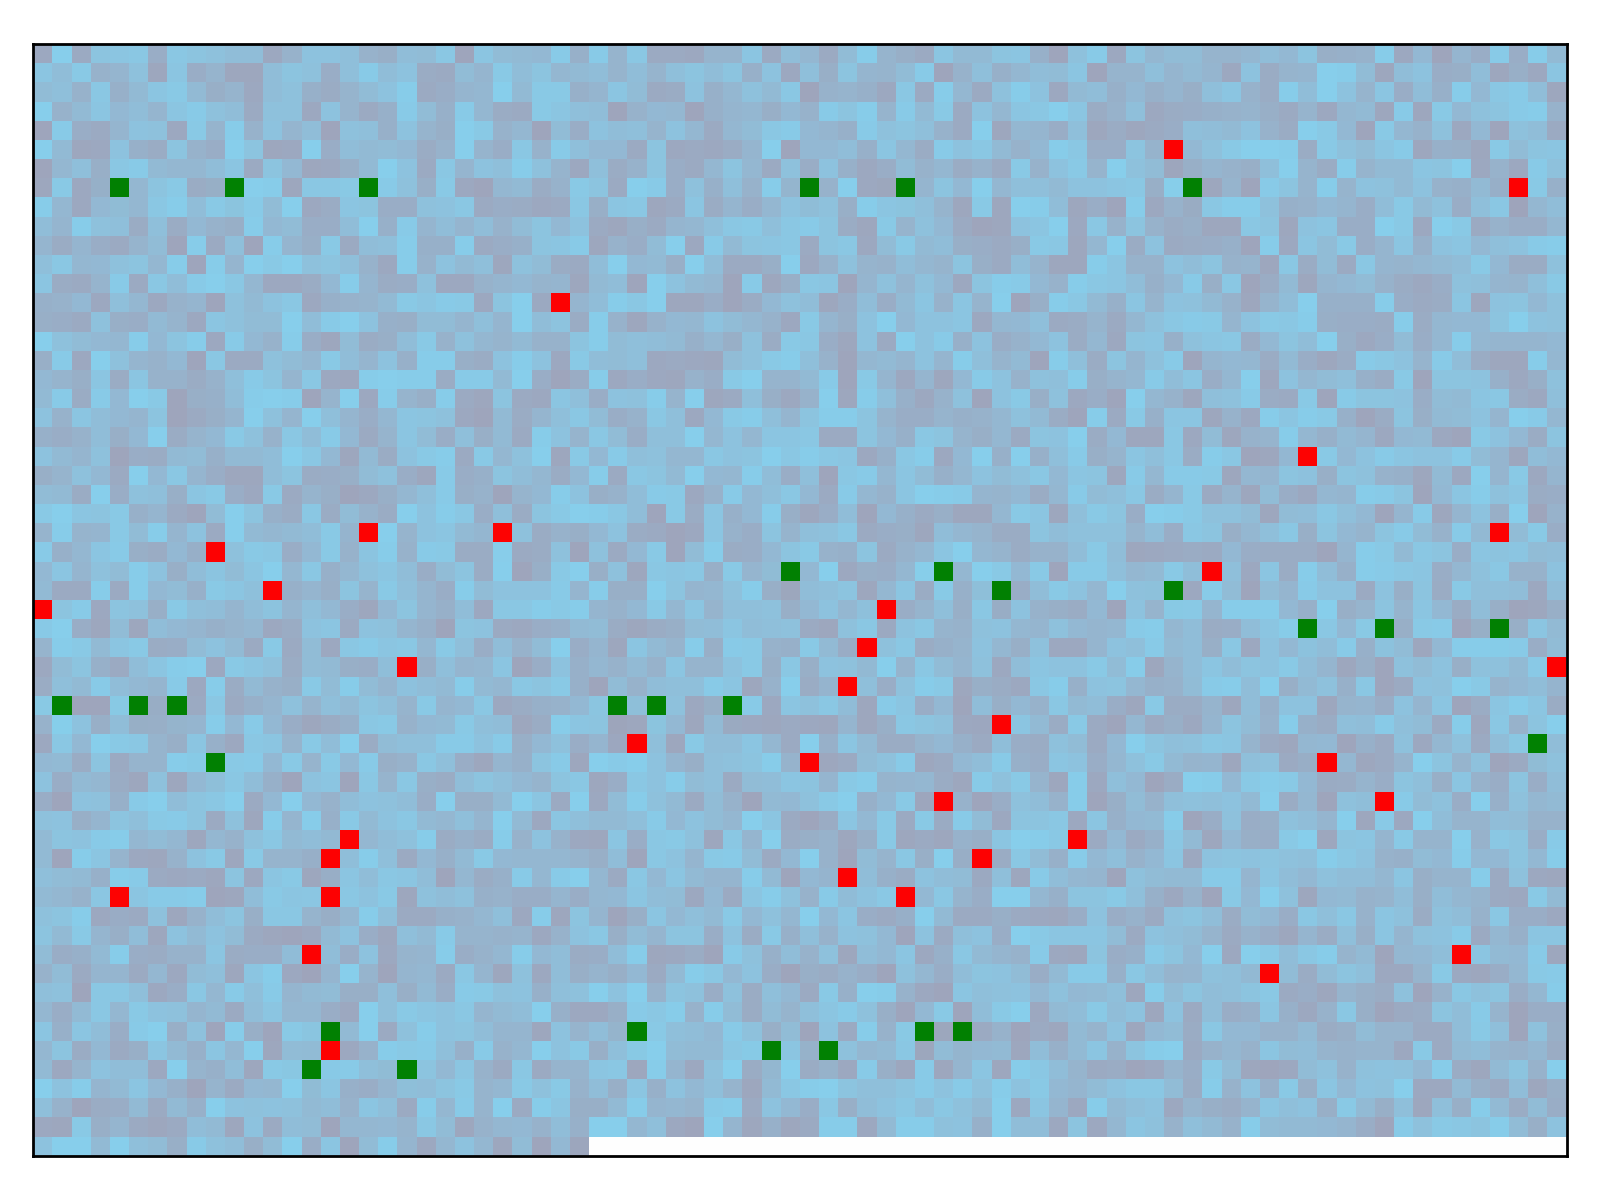
\includegraphics[width=0.75\textwidth]{doc11358_topic0.png} %&
        % 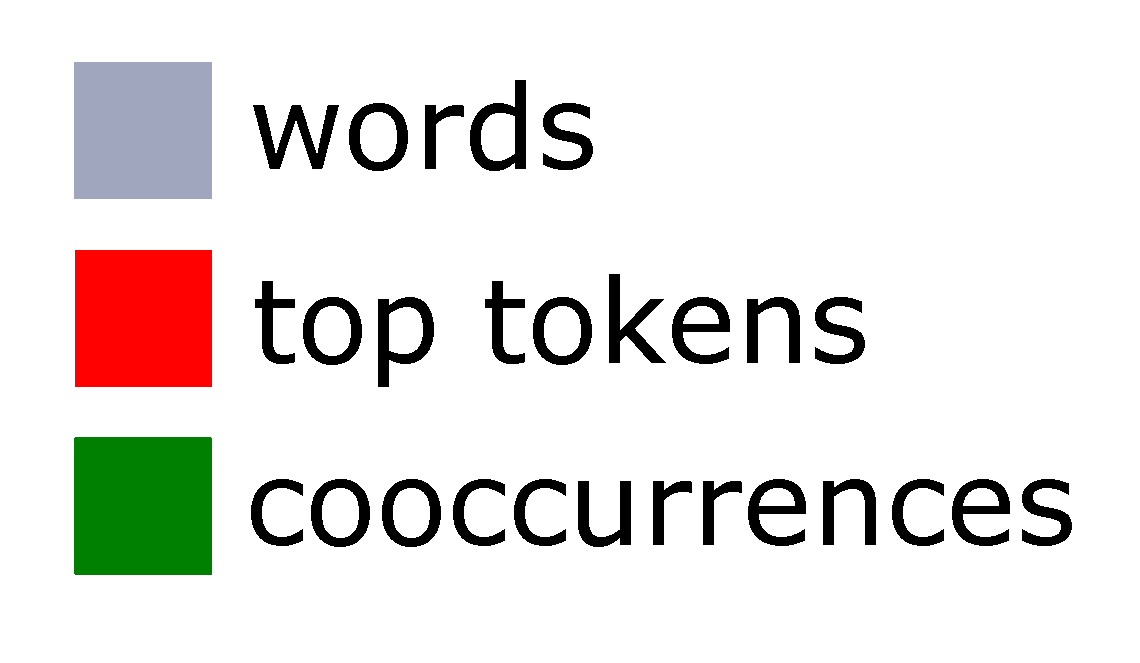
\includegraphics[width=0.25\textwidth]{legend.eps} \\
    %\end{tabular}
    \captionsetup{justification=raggedright,singlelinecheck=false,format=hang}
    \caption{Демонстрация доли текста, покрытой верхними словами, на примере одного документа. Словопозиции обозначены серо-синим цветом, словопозиции верхних слов показаны красным цветом, зелёным цветом показаны словопозиции, имеющие ненулевой вклад в расчёт когерентности (т.е. попадающие в скользящее окно вместе с другим верхним словом).}
\label{fig:ch3_doc_compound_auto}
\end{figure}

Также в этой главе предлагаются несколько мер качества, основанных на идее \textit{внутритекстовой когерентности}.
Традиционные меры когерентности сначала выделяют небольшое множество верхних слов в заданной теме по их $\phi_{wt}$ и затем анализируют, каким образом эти слова встречаются в тексте (анализ \emph{от темы к тексту}). В предлагаемом же методе сначала выделяются все соседние слова текста, распределение $\phi_{wt}$ которых затем анализируется (\emph{от текста к теме}).

Предполагается, что этот метод будет лучше характеризовать интерпретируемость тем, нежели традиционные меры когерентности. Эксперимент на полусинтетической коллекции показывает, что предлагаемый подход действительно отличается большей чувствительностью.

\underline{\textbf{В четвёртой главе}} рассматриваются способы увеличения интерпретируемости тематических моделей. Предложен метод подбора коэффициентов сглаживания, коэффициентов разреживания и весов дополнительных модальностей при помощи математического аппарата \textit{относительных коэффициентов}.

Эта техника облегчает построение тематических моделей, все темы которых различны и не <<загрязнены>> большим числом неинформативных токенов (слов общей лексики). Также она позволяет перенести имеющуюсся стратегию обучения тематической модели на другие текстовые коллекции схожей структуры.

Показано, что любому абсолютному коэффициенту сглаживания/разреживания $\Phi$ и $\Theta$ соответствует какой-то относительный коэффициент (и наоборот). Приводятся следующие формулы преобразований из $\lambda$ в $\tau$:

\begin{equation}
\tau = \frac{\lambda \sum_{d\in D} n_d }{(1-\lambda) |D| \cdot |T|} \label{sp_theta_rel2abs}
\end{equation}

\begin{equation}
\tau = \frac{n}{|T|\cdot|W|} \frac{\lambda}{(1-\lambda)}  \label{sp_phi_rel2abs}
\end{equation}

Регуляризатор сглаживания $\Theta$, воздействующий на темы $T$ и документы $D$, коэффициент $\tau$ которого вычислен по формуле \eqref{sp_theta_rel2abs}, можно проинтерпретировать как нахождение <<компромисса>>: результирующая $\Theta_{td}$ будет на $\lambda$ состоять из априорного распределения $\frac{1}{|T|}$ и на $(1-\lambda)$ из оценки максимума правдоподобия $\frac{n_{td}}{n_d}$.

Аналогично интерпретируется и формула \eqref{sp_phi_rel2abs} для регуляризатора сглаживания $\Phi$, воздействующего на темы $T$ и токены $W$. Здесь задаётся взвешенная комбинация из априорного распределения $\frac{1}{|W|}$ и оценки максимума правдоподобия $\frac{n_{wt}}{n_t}$.

Это означает, что любую существующую модель можно переформулировать в терминах относительного сглаживания и разреживания без каких-либо потерь. Практическая значимость этого результата заключается в вытекающей из него возможности переносить существующую схему сглаживания/разреживания на другую коллекцию схожей структуры.

Оставшаяся часть главы посвящена изучению роли матриц $\Phi$ и $\Theta$ в тематическом моделировании. Вопрос рассматривается с двух позиций: с точки зрения математической постановки задачи и с точки зрения построения и использования тематических моделей на практике. В терминах вероятностного смысла задачи обе матрицы являются равноправными.

При этом существует ряд причин, по которым естественно считать матрицу $\Theta$ второстепенной по отношению к $\Phi$. Особое значение для рассматриваемой работы имеет аргумент об интерпретируемости: описанный в предыдущей главе процесс оценки тем на интерпретируемость обычно состоит из выбора небольшого набора верхних слов для каждой темы и представления этого набора эксперту-человеку \cite{roder2015exploring}. В этом процессе используется только матрица $\Phi$. Таким образом, в контексте интерпретации найденных тем экспертами качество матрицы $\Phi$ оказывается более важным, чем качество матрицы $\Theta$.

В работе \cite{thetaless} доказывается, что введение функциональной зависимости $\Theta = f(\Phi)$ требует модификации EM-алгоритма. Эту модификацию можно истолковать, как добавление псевдорегуляризатора, что приводит к алгоритму быстрой векторизации документов на основании одной лишь матрицы $\Phi$. Именно в таком виде данный псевдорегуляризатор был интегрирован в открытую библиотеку TopicNet\footnote{\url{https://github.com/machine-intelligence-laboratory/TopicNet/blob/master/topicnet/demos/Topic-Thetaless-Regularizer.ipynb}}. 

Оставшаясся часть четвёртой главы посвящена изучению свойств этого псевдоргеуляризатора. Поведение модели с предложенным псевдоргеуляризатором исследуется на реальной текстовой коллекции. Результаты показывают, что этот псевдорегуляризатор действительно повышает ряд критериев качества, связанных с интерпретируемостью и успешно комбинируется с другими регуляризаторами.

\underline{\textbf{Пятая глава}} посвящена разработке библиотеке TopicNet. TopicNet --- открытая надстройка над библиотекой BigARTM, предоставляющая более удобные возможности для подбора гиперпараметров, для работы с пользовательскими регуляризаторами и для визуализации тематических моделей. Описанная библиотека доступна онлайн на GitHub.

Главная мотивация TopicNet --- создать инструмент, удобный как для новичков, так и для продвинутых пользователей. Большое внимание уделяется удобству работу и наличию <<рецептов моделирования>>, показывающих хорошее качество без трудоёмкой настройки гиперпараметров. Численный эксперимент показывает, что TopicNet с настройками <<по умолчанию>> превосходит модель LDA из открыто доступной библиотеки GenSim, также с настройками <<по умолчанию>>, по критериям различности, когерентности и информативности тем.

Библиотека TopicNet состоит из двух больших модулей: \texttt{Viewers} и \texttt{Cooking Machine}.  

Модуль \texttt{Viewers} содержит различные инструменты визуализации. Дизайн придерживается философии Unix: каждый вьювер имеет ограниченную область ответственности и способен возвращать результат операции в JSON-подобном виде.

Это даёт возможность комбинировать содержащиеся в модуле вьюверы, не теряя при этом удобные для конечного пользователя методы, возвращающие \texttt{pandas.DataFrame}, строку сформированного HTML, или отображающие результат сразу в ячейке вывода Jupyter Notebook. 

Модуль \texttt{Cooking Machine} содержит различные инструменты для моделирования, расположенные в иерархии основных классов. Эти классы отвечают за построение и обучение модели заданной структуры, за отбор моделей согласно заданным пользователем ограничениям, а также за сохранение, загрузку и журналирование происходящего процесса.

Процесс построения тематической модели представим в виде дерева. Каждый узел дерева содержит в себе тематическую модель, а ориентированные рёбра хранят информацию об отношениях <<предок-потомок>> вида <<модель $Y$ была получена из модели $X$ при помощи преобразования $T_{XY}$>>. Не все деревья эксперимента являются допустимыми. Мы накладываем ограничения на допустимые преобразования: требуем, чтобы все рёбра одного уровня описывали преобразования из одного и того же семейства, различающиеся лишь набором параметров. 

Одним из примеров таких преобразований является <<Применить к модели регуляризатор с произвольными параметрами>>. 

Класс \texttt{Experiment} отвечает за хранение, журналирование и актуализацию этой структуры.  

Все преобразования связаны с экземпляром класса \texttt{Cube}. Каждый \texttt{Cube} играет роль чертежа, задающего все преобразования на текущем уровне эксперимента. Таким образом, процесс обучения можно представить как цепочку кубов, последовательно соединённых друг с другом.  

Куб выполняет две важные функции. Первая --- это \textit{спецификация}: во время инициализации куб преобразует заданные пользователем параметры в многомерное пространство поиска. Вторая функция --- \textit{применение}: получив точку в пространстве поиска и тематическую модель, куб изменяет заданное множество параметров и/или гиперпараметров модели. Таким образом, он играет роль инкубатора для моделей, что отражено в названии класса. На Рис.  \ref{Training-scheme} приведена схема обучения, состоящая из двух кубов, применённых к одной модели.  

Классы \texttt{Experiment} и \texttt{Cube} позволяют сделать сложные стратегии обучения и журналирование экспериментов более сжатыми и доступными. Модуль \texttt{config\_parser} делает ещё один шаг в сторону облегчения конфигурируемости: стратегию обучения можно задать при помощи текстового конфигурационного файла в формате YAML.  

\begin{figure}[ht]
    \centering
    \captionsetup{justification=raggedright,singlelinecheck=false,format=hang}

    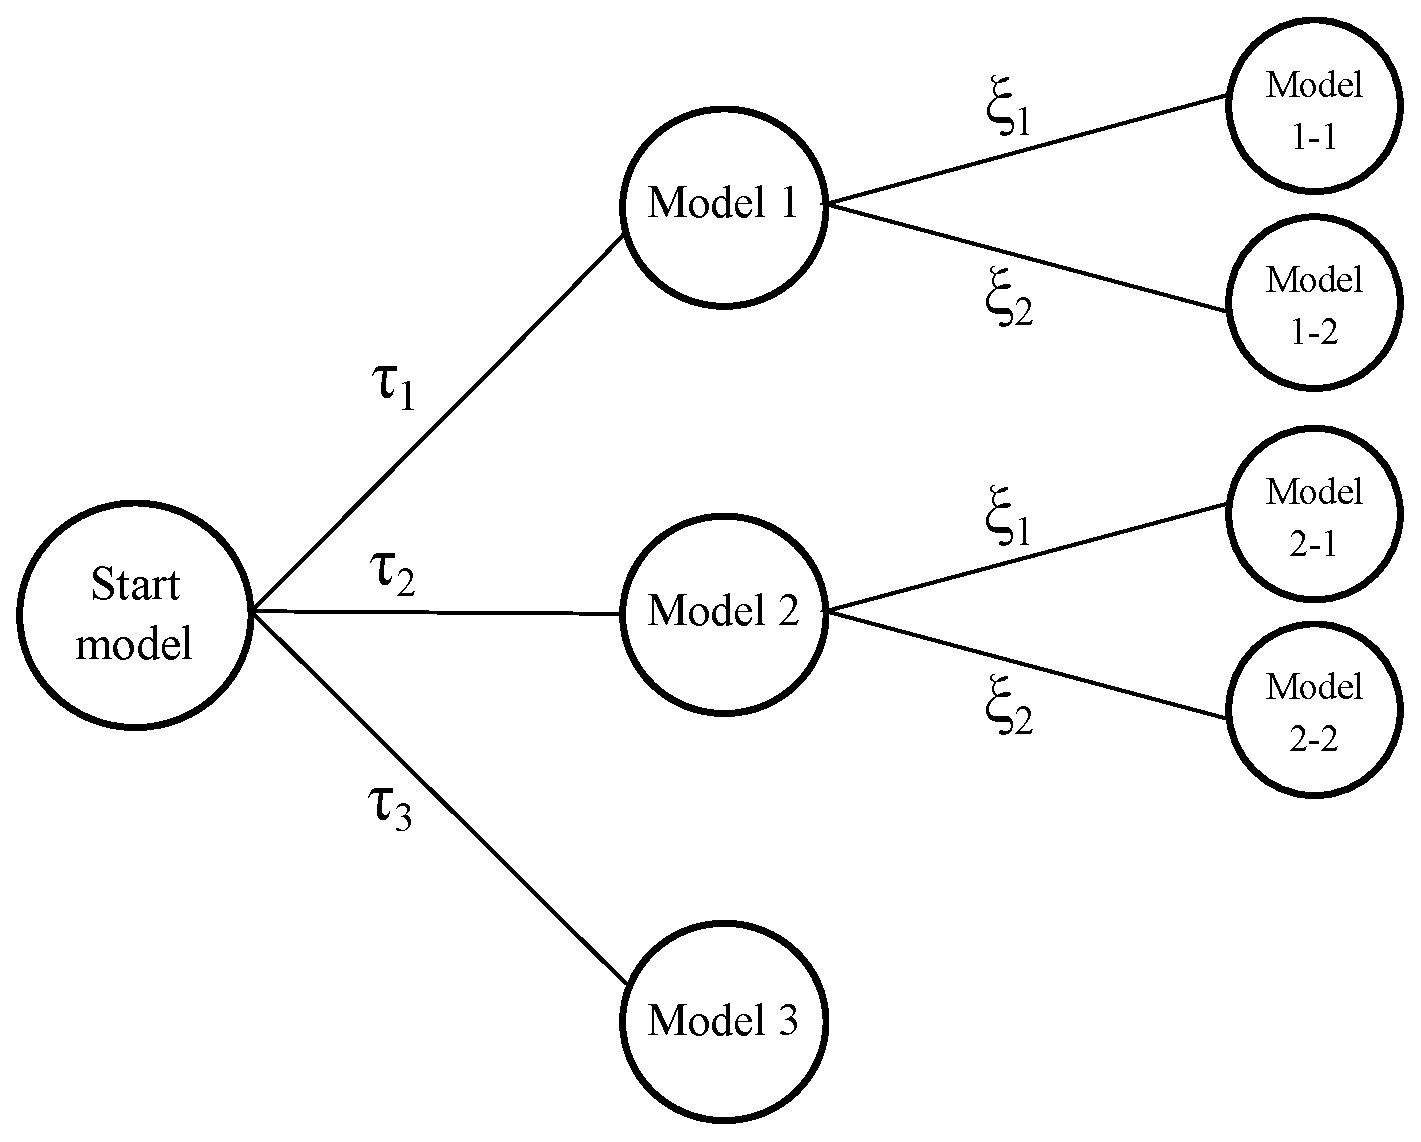
\includegraphics[width=0.7\textwidth]{training_scheme_example.eps}
    %\begin{flushleft}

    \caption{
        Пример двухэтапной схемы эксперимента.
        На первом этапе применяется регуляризатор с коэффициентом $\tau$, принимающим значения из некоторого множества $\{\tau_1, \tau_2, \tau_3\}$.
        Лучшими моделями после первого этапа являются \emph{Model 1} и \emph{Model 2}, поэтому \emph{Model 3} больше не участвует в процессе обучения.\\
        Второй этап связан с другим регуляризатором с коэффициентом $\xi$, принимающим значения из множества $\{\xi_1, \xi_2\}$.
        В результате этого этапа у каждой из ранее отобранных моделей  появляется два потомка.
    }
    %\end{flushleft}
\label{Training-scheme}
\end{figure} 


\begin{figure*}[ht]
% \footnotesize
\captionsetup{justification=raggedright,singlelinecheck=false,format=hang}
\texttt{TopicKernel@word.average\_contrast > 0.95 * MAXIMUM( \\
\hphantom{\ \ \ \ \ \ \ \ }TopicKernel@word.average\_contrast) \\
\hphantom{\ \ } and PerplexityScore@all < 1.1 * MINIMUM( \\
\hphantom{\ \ \ \ \ \ \ \ }PerplexityScore@all) \\
\hphantom{\ \ } and SparsityPhiScore@word -> max\\
\hphantom{\ \ } COLLECT 3} \\
\caption{Пример строки, задающей критерий отбора моделей. Здесь в качестве критериев отбора участвуют перплексия, контраст лексического ядра модальности \texttt{@word} и разреженность матрицы $\Phi$. Результатом будут три модели, контраст которых не более чем на 5\% отличается от наилучшего достигнутого контраста, имеют допустимую перплексию и как можно более разреженны. }
\label{DSL-example}
\end{figure*} 

В реальных экспериментах не у каждой модели есть потомки; большинство моделей отбрасывается в соответствии с каким-то критерием. Самый естественный, но в то же время самый трудозатратный способ анализа тематической модели --- это ручное изучение списков верхних токенов и верхних документов в темах, на основании которого пользователь принимает решение, какие из моделей являются <<удовлетворительными>>. Другой подход заключается в сравнении численных показателей; обычно используется перплексия и когерентность. Библиотека \mbox{BigARTM} добавляет к их числу дополнительные метрики разреженности, различности, чистоты и контрастности тем \cite{voron15mlj}, и другие.

Библиотека TopicNet также поддерживает пользовательские критерии качества. Значительная часть мер, описанных во второй главе, реализована на платформе TopicNet.  

Для того чтобы облегчить ручной анализ моделей, мы реализовали простой специализированный (domain-specific) язык для отбора моделей (пример приведён на Рис.~\ref{DSL-example}). Использование этого языка делает процесс многокритериального отбора моделей более простым и прозрачным.  

\underline{\textbf{В шестой главе}} рассматривается задача создания таксономии коллекции диалогов контактного центра без наличия разметки. Предлагается регуляризованная тематическая модель, играющая роль первого приближения к структуре коллекции.

Был использован усложнённый вариант распространённой техники, улучшающей интерпретируемость --- использования информативных $n$-грам (коллокаций) в качестве дополнительной модальности. Для того чтобы извлечь информативные $n$-грамы, был использован алгоритм TopMine~\cite{topmine}, основанный на статистике парной сочетаемости слов в текстовой коллекции.

Для нашей задачи имело смысл внести ряд правок в алгоритм TopMine. Во-первых, логика подсчёта статистик парной сочетаемости была модифицирована таким образом, чтобы в ней использовались мультимножества слов вместо последовательностей слов. 

Во-вторых, TopMine не выделяет пересекающиеся коллокации. Это приводит к тому, что похожие предложения (<<записать ребёнка в детский сад>> и <<записать ребёнка в детский садик>>) могут вовсе не содержать общих коллокаций. Примером служат предложение <<получение паспорта РФ>> (выделится коллокация \texttt{получение\_паспорт\_РФ}) и предложение <<паспорт РФ был утерян>> (выделится коллокация \texttt{паспорт\_РФ}). Это следует из процесса поиска коллокаций алгоритмом: на каждом шаге обработки соседние коллокации-кандидаты сливаются, если их объединение удовлетворяет критерию информативности. Для того чтобы устранить вышеописанную проблему, достаточно изменить процесс итеративного слияния фраз так, чтобы при успешном слиянии коллокаций они не удалялись из множества кандидатов. Данная модификация увеличивает потребление памяти алгоритмом, однако делает процесс поиска менее <<жадным>>.

% Во-первых, исходный алгоритм вычисляет статистики совстречаемости для упорядоченных кортежей слов $(w_1, w_2, \dots, w_k)$. В частности, алгоритм различает последовательности $(w_1, w_2)$ и $(w_2, w_1)$. Эта особенность делает алгоритм TopMine плохо приспособленными для обработки текстов на языках с нестрогим порядком слов (таких как русский). По этой причине логика подсчёта статистик совстречаемостей алгоритма была модифицирована таким образом, чтобы в ней использовались мультимножества слов вместо последовательностей слов.

Предлагаемая модель является двухуровневой, то есть состоит из двух <<обычных>> тематических моделей. Модель первого уровня и модель второго ориентируются на различные признаки. Это связано с тем, что первый уровень иерархии предназначен для определения предмета диалога, а цель второго уровня иерархии --- нахождение действий, о которых говорит пользователь. % Существительные имеют большое влияние на темы первого уровня, а для тем второго уровня более важную роль играют глаголы.

В контексте поставленной задачи было предпринято разделение признаков по их функциональному назначению. Из всех токенов (слов и $n$-грам) были выделены две группы на основании их частеречного состава: <<тематическая>> и <<функциональная>>. <<Функциональная>> группа состоит из одиночных глаголов и $n$-грам, содержащих хотя бы один глагол. <<Тематическая>> группа состоит из одиночных существительных, одиночных прилагательных и $n$-грамм, включающих в себя хотя бы одно существительное и не имеющих в своём составе глаголов.

Таким образом, предлагаемая тематическая модель использует пять модальностей: \texttt{@lemmatized} (просто слова), \texttt{@verb\_lemmatized} (слова-глаголы), \texttt{@noun\_lemmatized} (слова-существительные и слова-прилагательные), \texttt{@theme\_ngramms} ($n$-грамы с существительными и без глаголов), \texttt{@verb\_ngramms} ($n$-грамы с глаголами).

Одна и та же стратегия обучения успешно применяется к двум разным коллекциям диалогов. Первая коллекция состоит из диалогов клиентов с представителями различными государственных организаций, а вторая представляет собой логи технической поддержки провайдера. Механизм относительных коэффициентов позволил успешно перенести веса модальностей, подобранные на первой коллекции, на вторую коллекцию.

\FloatBarrier
\pdfbookmark{Заключение}{conclusion}                                  % Закладка pdf
В \underline{\textbf{заключении}} приведены основные результаты работы, которые заключаются в следующем:
%% Согласно ГОСТ Р 7.0.11-2011:
%% 5.3.3 В заключении диссертации излагают итоги выполненного исследования, рекомендации, перспективы дальнейшей разработки темы.
%% 9.2.3 В заключении автореферата диссертации излагают итоги данного исследования, рекомендации и перспективы дальнейшей разработки темы.
\begin{enumerate}[beginpenalty=10000]
\item
    Методология построения аддитивно регуляризованных тематических моделей, обеспечивающая формирование <<рецептов моделирования>> с автоматизированным подбором гиперпараметров по множеству критериев и отличающаяся использованием относительных коэффициентов регуляризации и кубов гиперпараметров.
\item
    Архитектура библиотеки TopicNet, обеспечивающая программную реализацию данной методологии и отличающаяся использованием удобного языка описания кубов гиперпараметров и возможностью создания пользовательских регуляризаторов и метрик качества на языке Python.
\item
    Универсальный рецепт моделирования, обеспечивающий многокритериальный выбор тематических моделей для широкого класса задач, отличающийся предварительной настройкой куба гиперпараметров по набору разнородных задач тематического моделирования.
\item
    Программная реализация нового критерия когерентности, обеспечивающая его эффективное вычисление и отличающаяся более полным использованием данных о сочетаемости слов внутри текстовых документов.
%\item
%    Программная реализация псевдорегуляризатора в библиотеке TopicNet, обеспечивающего быстрое однопроходное вычисление тематических векторных представлений документов и улучшение качества тематической модели по множеству критериев.
\end{enumerate}




\pdfbookmark{Литература}{bibliography}                                % Закладка pdf

% При использовании пакета \verb!biblatex! список публикаций автора по теме диссертации формируется в разделе <<\publications>>\ файла \verb!common/characteristic.tex!  при помощи команды \verb!\nocite!

\ifdefmacro{\microtypesetup}{\microtypesetup{protrusion=false}}{} % не рекомендуется применять пакет микротипографики к автоматически генерируемому списку литературы
\urlstyle{rm}                               % ссылки URL обычным шрифтом
\ifnumequal{\value{bibliosel}}{0}{% Встроенная реализация с загрузкой файла через движок bibtex8
  \renewcommand{\bibname}{\large \bibtitleauthor}
  \nocite{*}
  \insertbiblioauthor           % Подключаем Bib-базы
  %\insertbiblioexternal   % !!! bibtex не умеет работать с несколькими библиографиями !!!
}{% Реализация пакетом biblatex через движок biber
  % Цитирования.
  %  * Порядок перечисления определяет порядок в библиографии (только внутри подраздела, если `\insertbiblioauthorgrouped`).
  %  * Если не соблюдать порядок "как для \printbibliography", нумерация в `\insertbiblioauthor` будет кривой.
  %  * Если цитировать каждый источник отдельной командой --- найти некоторые ошибки будет проще.
  %
  \nocite{intracoh, popov_hier, bulatov2020topicnet, thetaless}

  %% authorprogram
  \nocite{prog_cook}%
  \nocite{prog_stkc}%
  \nocite{prog_view}%
  %

  \ifnumgreater{\value{usefootcite}}{0}{
    \begin{refcontext}[labelprefix={}]
      \ifnum \value{bibgrouped}>0
        \insertbiblioauthorgrouped    % Вывод всех работ автора, сгруппированных по источникам
      \else
        \insertbiblioauthor      % Вывод всех работ автора
      \fi
    \end{refcontext}
  }{
  \ifnum \totvalue{citeexternal}>0
    \begin{refcontext}[labelprefix=A]
      \ifnum \value{bibgrouped}>0
        \insertbiblioauthorgrouped    % Вывод всех работ автора, сгруппированных по источникам
      \else
        \insertbiblioauthor      % Вывод всех работ автора
      \fi
    \end{refcontext}
  \else
    \ifnum \value{bibgrouped}>0
      \insertbiblioauthorgrouped    % Вывод всех работ автора, сгруппированных по источникам
    \else
      \insertbiblioauthor      % Вывод всех работ автора
    \fi
  \fi
  %  \insertbiblioauthorimportant  % Вывод наиболее значимых работ автора (определяется в файле characteristic во второй section)
  \begin{refcontext}[labelprefix={}]
      \insertbiblioexternal            % Вывод списка литературы, на которую ссылались в тексте автореферата
  \end{refcontext}
  
  % Невидимый библиографический список для подсчёта количества внешних публикаций
  % Используется, чтобы убрать приставку "А" у работ автора, если в автореферате нет
  % цитирований внешних источников.
  % \printbibliography[heading=nobibheading, section=1, keyword=biblioexternal]%
  }
}
\ifdefmacro{\microtypesetup}{\microtypesetup{protrusion=true}}{}
\urlstyle{tt}                               % возвращаем установки шрифта ссылок URL
